
\documentclass[12pt]{article}
 
\usepackage[margin=1in]{geometry} 
\usepackage{amsmath,amsthm,amssymb}
\usepackage{pifont}
\usepackage{graphics}
\usepackage{graphicx}
\usepackage{array}
 
\newcommand{\N}{\mathbb{N}}
\newcommand{\Z}{\mathbb{Z}}
 
\newenvironment{theorem}[2][Theorem]{\begin{trivlist}
\item[\hskip \labelsep {\bfseries #1}\hskip \labelsep {\bfseries #2.}]}{\end{trivlist}}
\newenvironment{lemma}[2][Lemma]{\begin{trivlist}
\item[\hskip \labelsep {\bfseries #1}\hskip \labelsep {\bfseries #2.}]}{\end{trivlist}}
\newenvironment{exercise}[2][Exercise]{\begin{trivlist}
\item[\hskip \labelsep {\bfseries #1}\hskip \labelsep {\bfseries #2.}]}{\end{trivlist}}
\newenvironment{problem}[2][Problem]{\begin{trivlist}
\item[\hskip \labelsep {\bfseries #1}\hskip \labelsep {\bfseries #2.}]}{\end{trivlist}}
\newenvironment{question}[2][Question]{\begin{trivlist}
\item[\hskip \labelsep {\bfseries #1}\hskip \labelsep {\bfseries #2.}]}{\end{trivlist}}
\newenvironment{corollary}[2][Corollary]{\begin{trivlist}
\item[\hskip \labelsep {\bfseries #1}\hskip \labelsep {\bfseries #2.}]}{\end{trivlist}}

\newenvironment{solution}{\begin{proof}[Solution]}{\end{proof}}
 
\begin{document}
 
% --------------------------------------------------------------
%                         Start here
% --------------------------------------------------------------
 
\title{Homework 1}
\author{Georgios Kontoudis\\ 
ME6544 Linear Control Theory\\
Professor Kyriakos Vamvoudakis} 
\date{Spring 2018}
 
\maketitle
\begin{problem}{1.1.1} %theorem, exercise, problem, or question 
RLC state space
\end{problem}
\begin{solution}

By using the first Kirchoff's law $\sum_n i_n= 0$ we obtain 
\begin{equation}\label{eq_KVL}
\begin{aligned}
& i_0
& =
&&& i_1+i_2\\
&& =
&&& i_C+i_{R_2}\\
&& =
&&& C \frac{dV_C}{dt}+\frac{V_{R_2}}{R_2}.
\end{aligned}
\end{equation}
Next, for the first closed loop the second Kirchoff's law $\sum_n u_n= 0$  yields
\begin{equation}\label{eq_KIL1}
\begin{aligned}
& V_0
& =
&&& V_{R_1}+V_L+V_C\\
&& =
&&& R_1i_0+L\frac{di_0}{dt}+V_C,
\end{aligned}
\end{equation}
and for the second closed loop
\begin{equation}\label{eq_KVL2}
\begin{aligned}
& V_C
& =
&&& V_{R_2}.
\end{aligned}
\end{equation}

Considering that the state vector is $\textbf{x}=[i_0 \hspace{.2cm} V_C]^T$, the input is $u=V_0$, and the output is $y=V_{R_2}$, and by employing Equations~\ref{eq_KVL}, \ref{eq_KVL2} we get 
\begin{equation}\label{eq_x2}
\begin{aligned}
& x_1
& =
&&& C\dot{x_2}+\frac{x_2}{R_2}\\
& \dot{x_2}
& =
&&& \frac{1}{C}x_1-\frac{1}{CR_2}x_2.
\end{aligned}
\end{equation}
Then, Equation~\ref{eq_KIL1} results
\begin{equation}\label{eq_x1}
\begin{aligned}
& u
& =
&&& R_1x_1+L\dot{x_1}+x_2\\
& \dot{x_1}
& =
&&& -\frac{R_1}{L}x_1-\frac{1}{L}x_2+\frac{1}{L}u.
\end{aligned}
\end{equation}
Next, Equation~\ref{eq_KVL2} reveals the output
\begin{equation}\label{eq_y}
\begin{aligned}
& y
& =
&&& x_2.
\end{aligned}
\end{equation}
 
By employing Equations~\ref{eq_x2}, \ref{eq_x1}, \ref{eq_y} we obtain the state space form 

\begin{equation*}
\begin{aligned}
& \begin{bmatrix}
\dot{x_1} \\ \dot{x_2}
\end{bmatrix}
&  =
&&& \begin{bmatrix}
-\frac{R_1}{L} & -\frac{1}{L} \\
\frac{1}{C} & -\frac{1}{CR_2}
\end{bmatrix}
\begin{bmatrix}
x_1 \\
x_2
\end{bmatrix}+
\begin{bmatrix}
\frac{1}{L} \\
0
\end{bmatrix}
u\\
& y
&  =
&&& \begin{bmatrix}
0  & 1
\end{bmatrix}
\begin{bmatrix}
x_1 \\
x_2
\end{bmatrix}
\end{aligned}
\end{equation*}
\end{solution}



\begin{problem}{1.1.2} %theorem, exercise, problem, or question
RLC
\end{problem}
\begin{solution}
The selected resistance values are $R=\{ .1, .5, 3, 20 \}$, the inductance values are $L=\{1 , .3, 6 , 15 \}$, and the capacitance values are $C=\{10 , 5, 1 , 2 \}$. In Figures~\ref{fig_state1}, \ref{fig_state2} the state trajectories  $x_1(t)$, $x_2(t)$ for various R, L, C values are presented respectively. In Figure~\ref{fig_output} the output trajectory $y(t)$ for various R, L, C values are depicted. In Figure~\ref{fig_phase} the phase of the states $x_1$, $x_2$ for various R, L, C values are illustrated.
  
\begin{figure}[!h]
	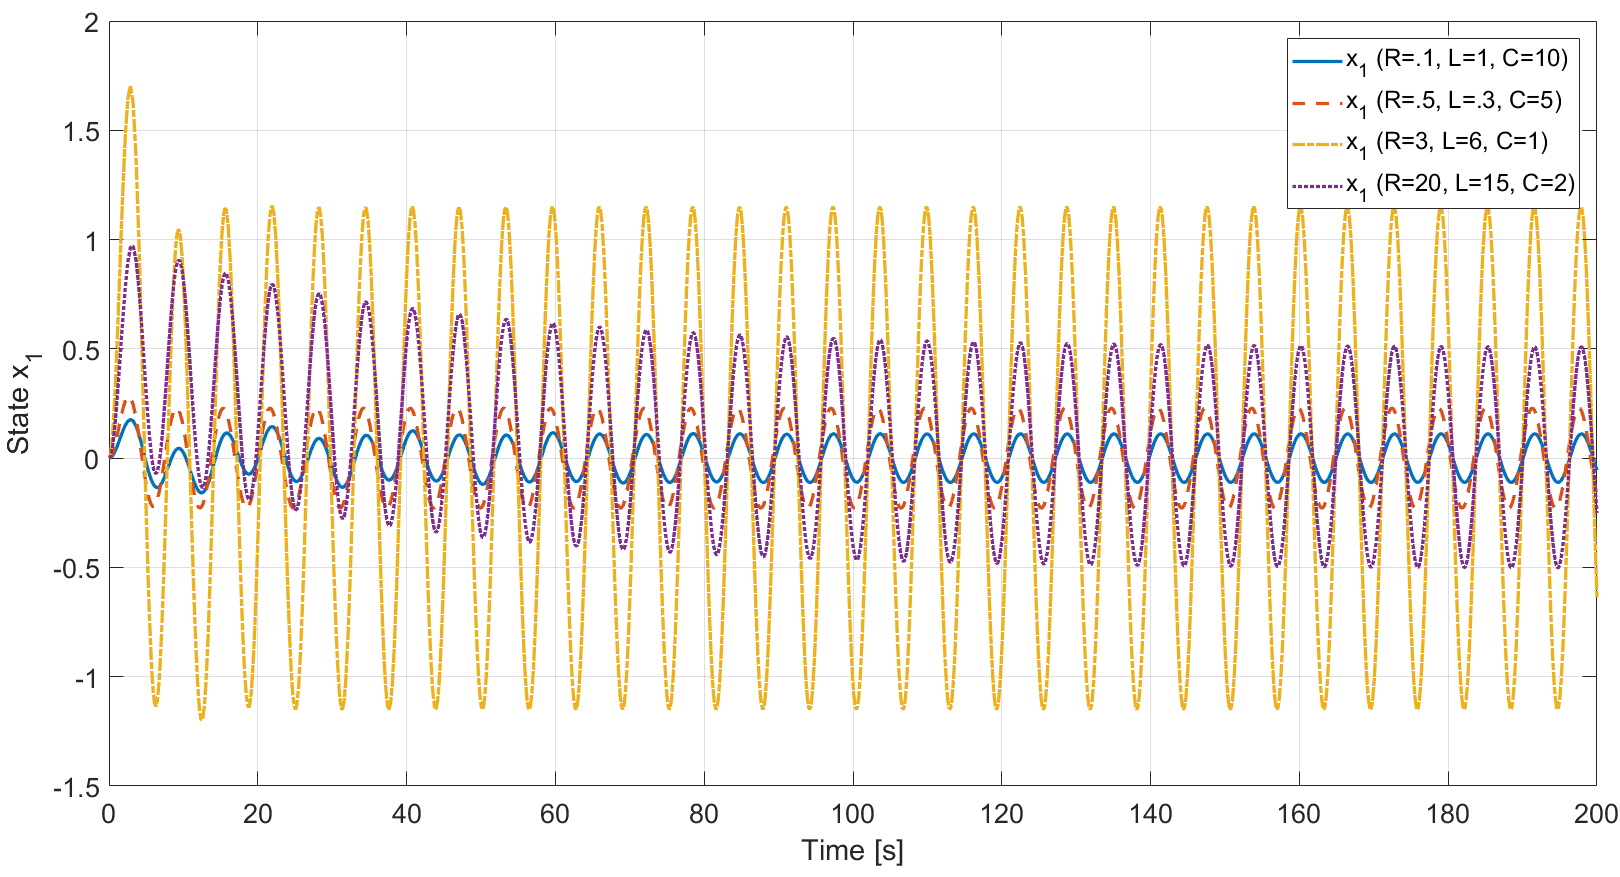
\includegraphics[width=.9\columnwidth]{figures/1_1_2_state_1.png}
	\centering
	\caption{The state $x_1$ trajectory for various R, L, C values.}
	\label{fig_state1}
\end{figure}
\begin{figure}[!h]
	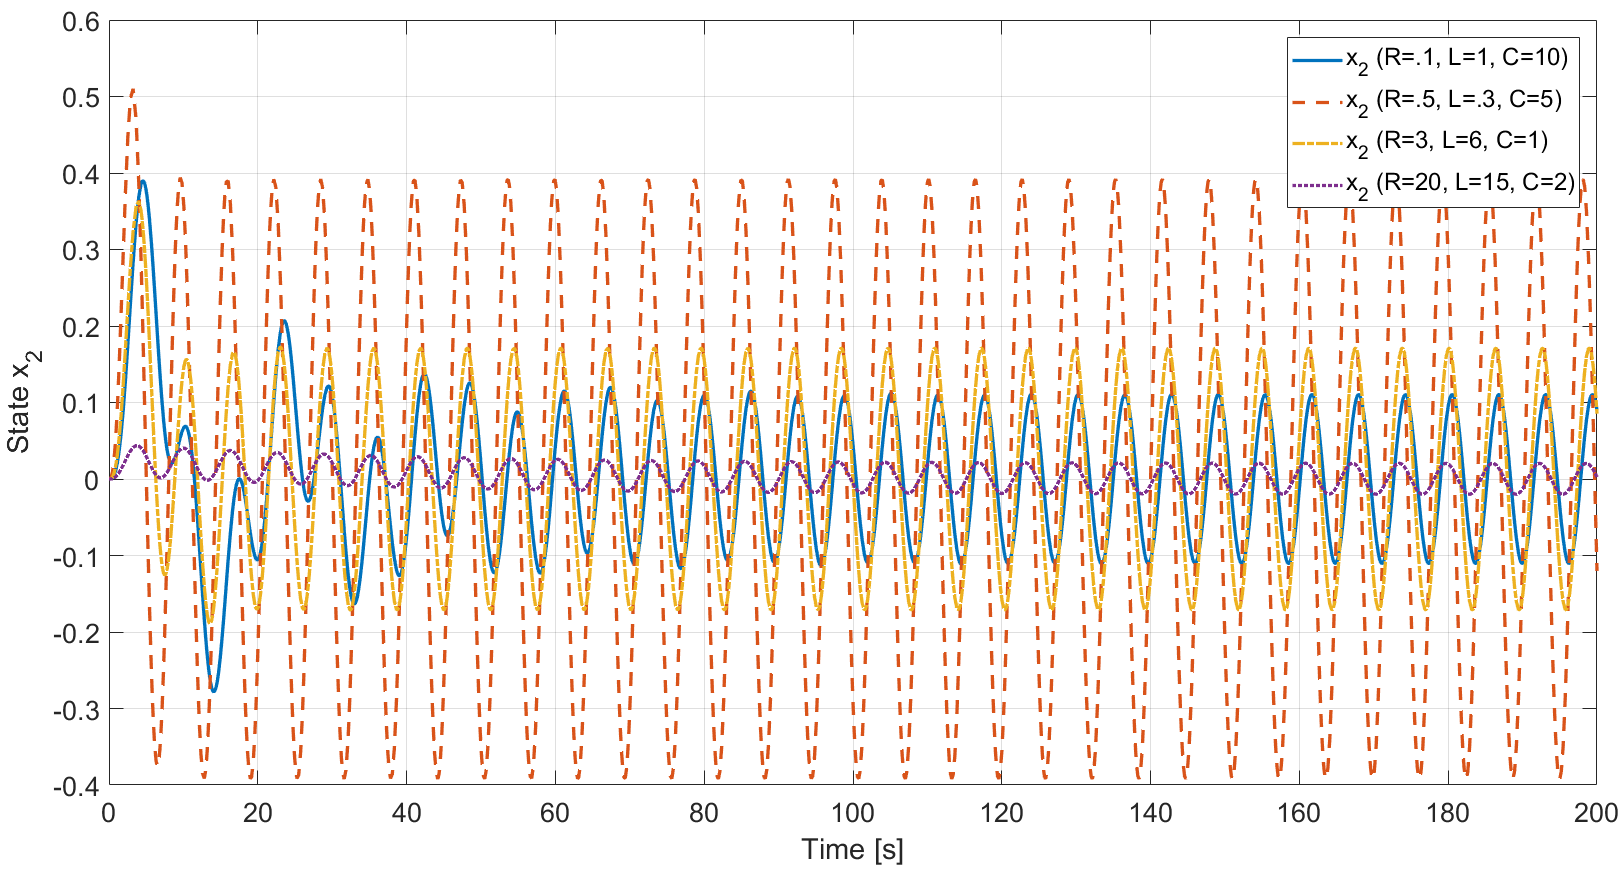
\includegraphics[width=.9\columnwidth]{figures/1_1_2_state_2.png}
	\centering
	\caption{The state $x_2$ trajectory for various R, L, C values.}
	\label{fig_state2}
\end{figure}
\begin{figure}[!h]
	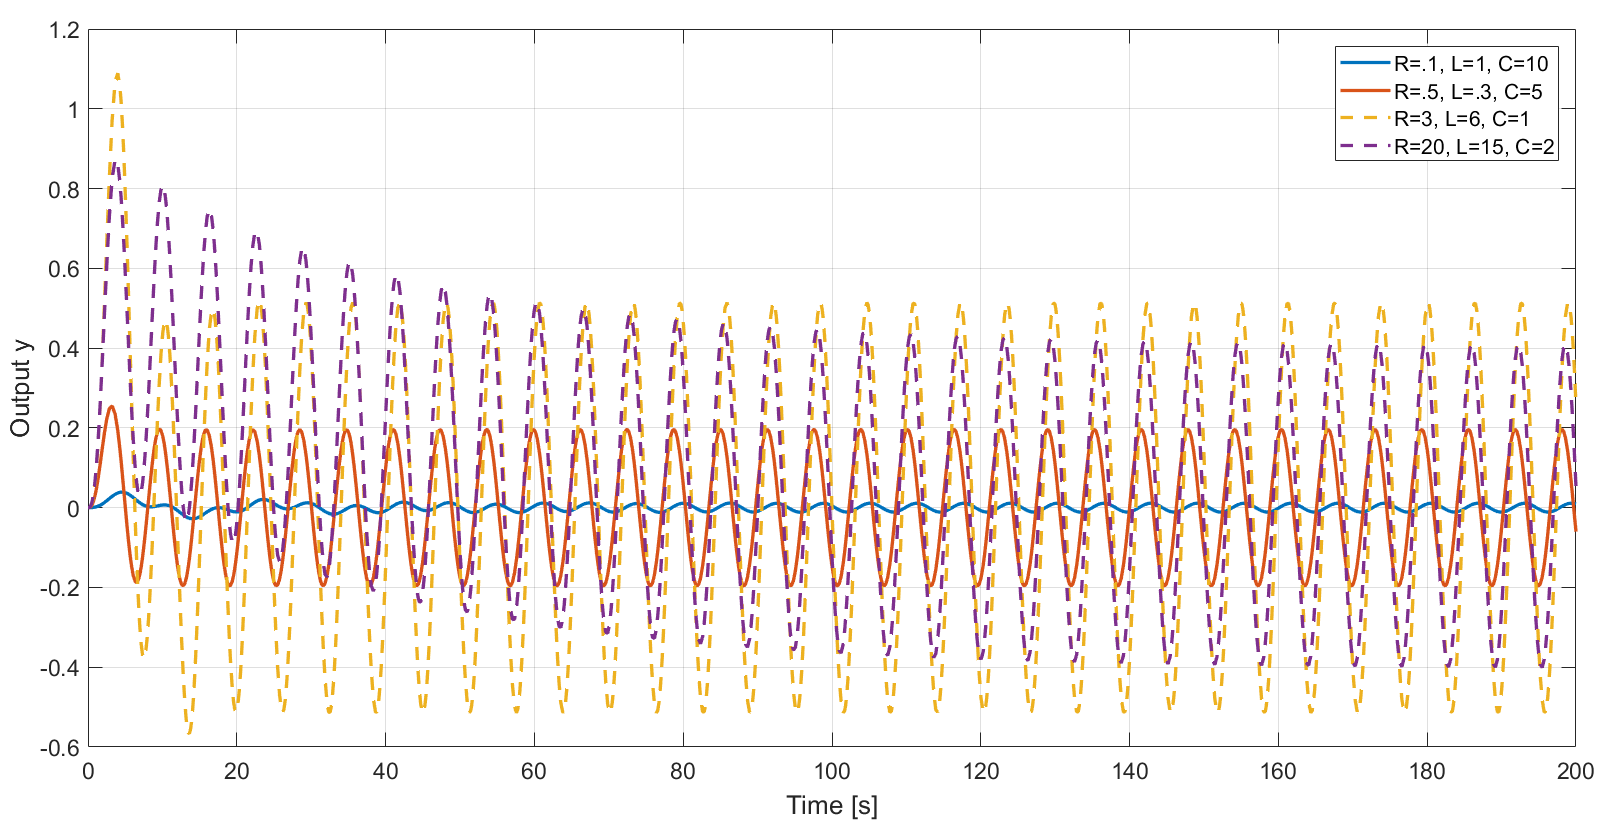
\includegraphics[width=.9\columnwidth]{figures/1_1_2_outputPlot.png}
	\centering
	\caption{The output trajectories for various R, L, C values.}
	\label{fig_output}
\end{figure}
\begin{figure}[!h]
	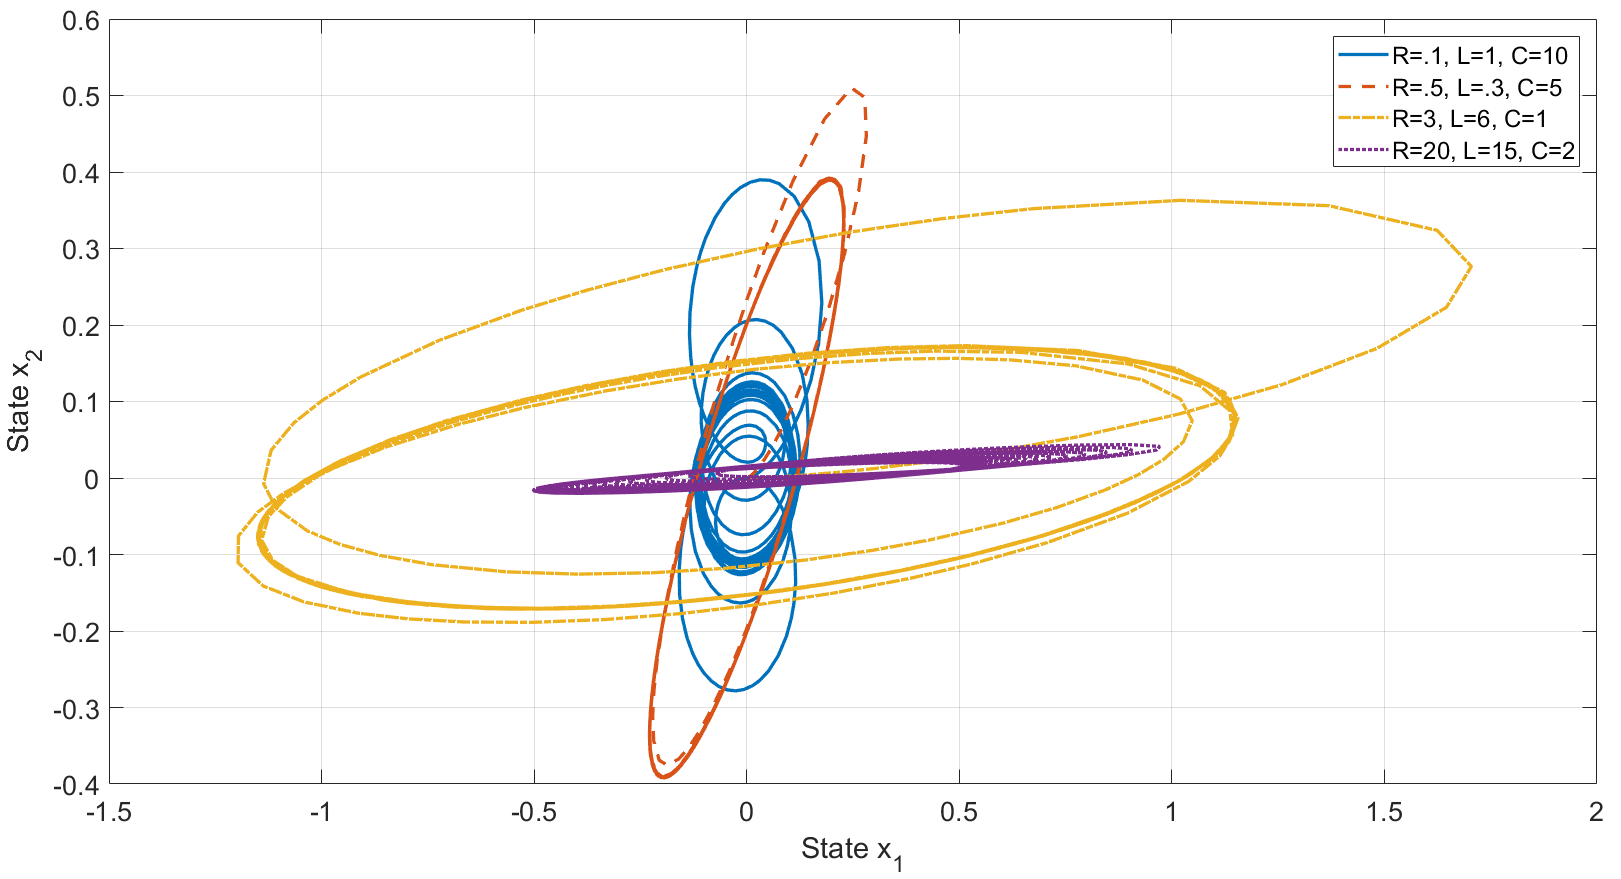
\includegraphics[width=.9\columnwidth]{figures/1_1_2_phasePlot.png}
	\centering
	\caption{The phase of the states $x_1$, $x_2$ for various R, L, C values.}
	\label{fig_phase}
\end{figure}

The state $x_1$ is only affected by the capacitance $C$ as depicted in Figure~\ref{fig_state1}. More specifically as $C$ increases the magnitude of the state $x_1$ decreases. The periodic performance is imposed by the input. The state $x_2$ is affected by a combination of the capacitance $C$, the resistance $R$, and the inductance $L$ as shown in Figure~\ref{fig_state2}. More specifically, as the inductance $L$ increases the magnitude of the state $x_2$ decreases. Next, as the fraction $\frac{R}{C}$ increases the magnitude of the state $x_2$ decreases. The periodic performance is imposed by the state $x_1$. The phase of the states $x_1$, $x_2$ performance is a combination of the aforementioned factors that affect the states $x_1$, $x_2$ as shown in Figure~\ref{fig_phase}. Finally, the output $y$ has similar performance with the state $x_2$, but it is also proportional with the resistance $R$ as presented in Figure~\ref{fig_output}.

\end{solution}

\begin{problem}{1.2} %theorem, exercise, problem, or question 
Van Der Pol Oscillator
\end{problem}
\begin{solution}
The forced Van der Pol oscillator is described by
\begin{equation}\label{eq_vdpSingle}
\begin{aligned}
& \ddot{y}-\mu (1-y^2)\dot{y}+y-A\sin{\omega t}
& =
&&& 0.
\end{aligned}
\end{equation}
It cannot be expressed in state space form because it includes non-linearities such as cross term multiplications and variables in raised powers. More specifically, it is a second order, autonomous, non-linear differential equation. Although, for the simulation we can derive the first order differential equations
\begin{equation}\label{eq_vdp}
\begin{aligned}
& \dot{y_1}
& =
&&& y_2\\
& \dot{y_2}
& =
&&& \mu(1-y_1^2)y_2-y_1+u,
\end{aligned}
\end{equation}
where $u=A\sin{\omega t}$ is a periodic input. For the given initial conditions $y(0)=0$, $\dot{y}=0.5$ the trajectory $y(t)$ is shown in Figure~\ref{fig_vdp}, and the phase plane for ($\dot{y}$, $y$) is presented in Figure~\ref{fig_vdpPhase}. 
\begin{figure}[!h]
	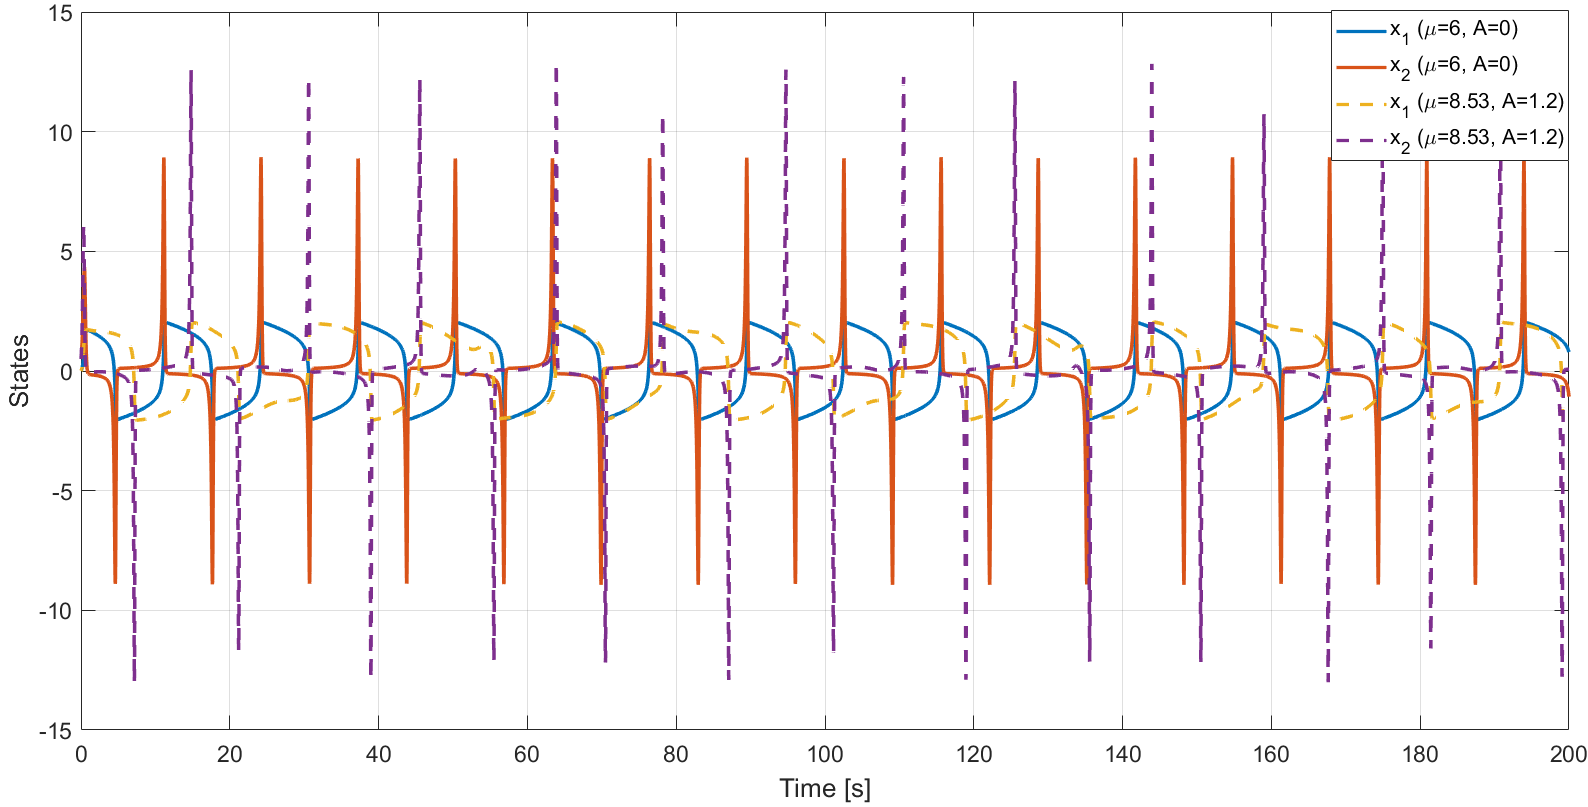
\includegraphics[width=.8\columnwidth]{figures/1_2_VanDerPol.png}
	\centering
	\caption{Van der Pol oscillator trajectories.}
	\label{fig_vdp}
\end{figure}
\begin{figure}[!h]
	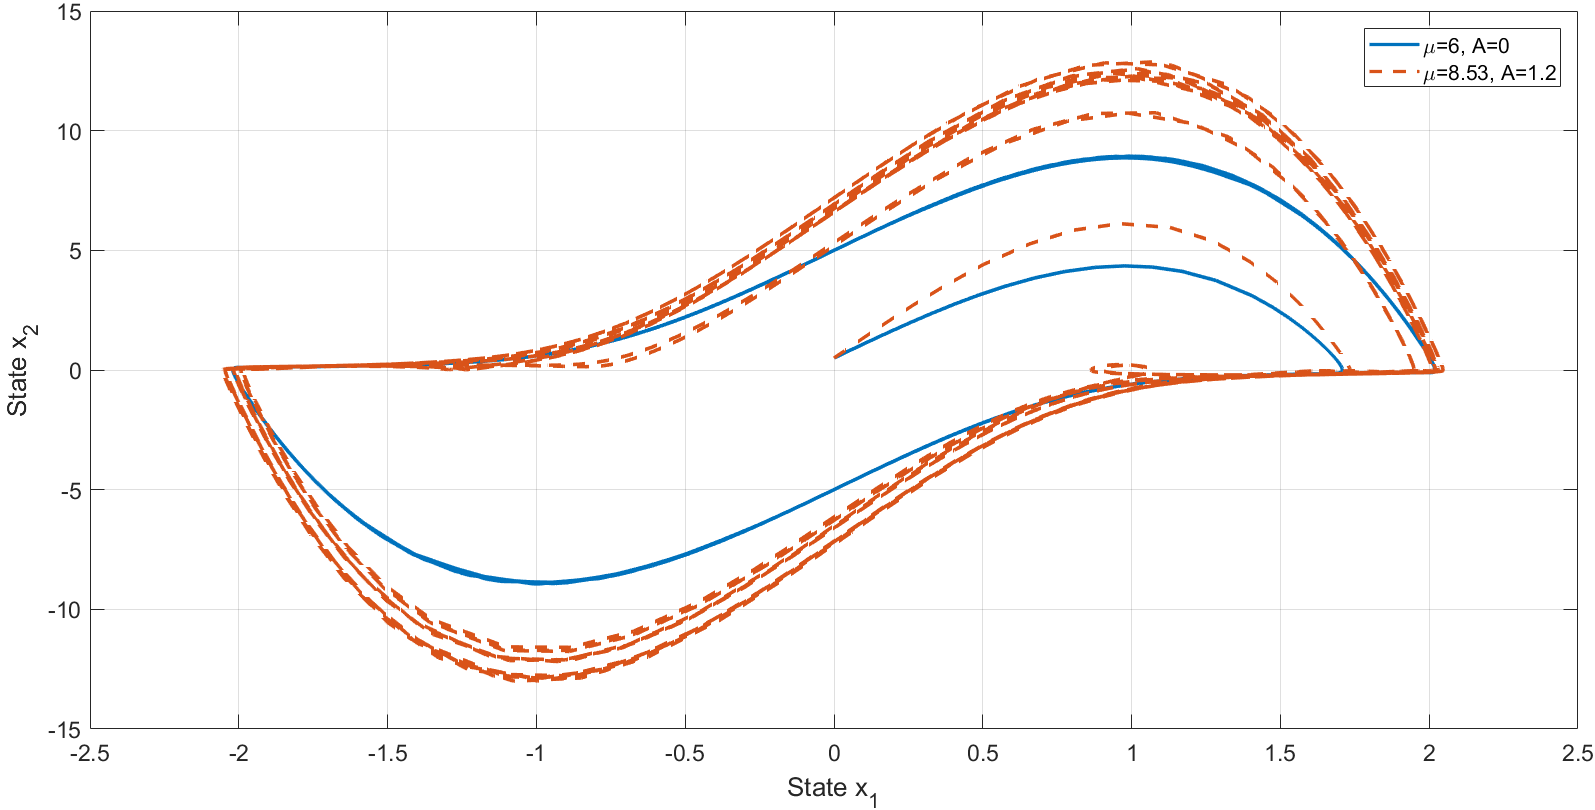
\includegraphics[width=.8\columnwidth]{figures/1_2_VanDerPol_phase.png}
	\centering
	\caption{Van der Pol oscillator phase of states $x_1$, $x_2$.}
	\label{fig_vdpPhase}
\end{figure}

\end{solution}

\begin{problem}{1.3} %theorem, exercise, problem, or question 
Block Diagram and State Evolution
\end{problem}
\begin{solution}
The block diagram is presented in Figure~\ref{fig_blockDiagram}.
\begin{figure}[!h]
	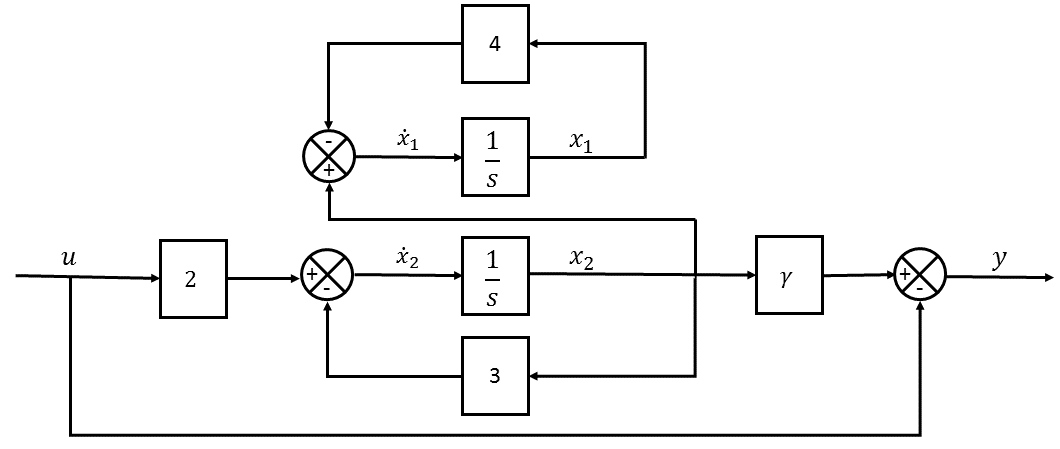
\includegraphics[width=.8\columnwidth]{figures/1_3_blockDiagram.png}
	\centering
	\caption{Block diagram of the given system.}
	\label{fig_blockDiagram}
\end{figure}
The given system relates the output with the input as
\begin{equation}\label{eq_outputSE}
\begin{aligned}
& y
& =
&&& \gamma x_2 -u,
\end{aligned}
\end{equation}
where $u$ is the input, $y$ is the output, and $x_2$ is a state. Ideally, we want to conceive a way to express the input and the output without any state correlation. For this reason, we compute the time derivative of Equation~\ref{eq_outputSE} which yields
\begin{equation}\label{eq_derOutpout}
\begin{aligned}
& \dot{y}
& =
&&& \gamma \dot{x_2} -\dot{u}.
\end{aligned}
\end{equation}
Then, we substitute the second state from the state space description
\begin{equation}\label{eq_derOutpout2}
\begin{aligned}
& \dot{y}
& =
&&& \gamma (-3x_2 +2u) -\dot{u}\\
&& =
&&& -3 \gamma x_2 +2\gamma u - \dot{u}.
\end{aligned}
\end{equation}
Next, we employ Equation~\ref{eq_outputSE} to eliminate the state $x_2$, which results to a first order ordinary differential equation
\begin{equation}\label{eq_derOutpout_final}
\begin{aligned}
&& \dot{y}
 =
&&& -3 \gamma (\frac{y+u}{\gamma}) +2\gamma u - \dot{u}\\
&& \dot{y}
 =
&&& -3 y+ -3u + 2\gamma u - \dot{u}\\
&& \dot{y}+3y
 =
&&& u(2\gamma-3) - \dot{u}.
\end{aligned}
\end{equation}

\end{solution}

\begin{problem}{1.4} %theorem, exercise, problem, or question 
Transfer Function
\end{problem}
\begin{solution}
For the $3D$ magnitude and phase plots we need to express the open loop transfer function with respect to the real and the imaginary parts. The given transfer function has one zero at $z=-6$ and 2 conjugate complex poles at $p_1=-2.5+j2.5981$, $p_2=-2.5-j2.5981$, which yields
\begin{equation}\label{eq_transferFunc}
\begin{aligned}
& H(s)
& =
&&& \frac{s+6}{s^2+5s+13}\\
& H(s)
& =
&&& \frac{s+6}{(s+2.5-2.5981j)(s+2.5+2.5981j)}.
\end{aligned}
\end{equation}
Then, we substitute to Equation~\ref{eq_transferFunc} the complex number $s=a+bj$ to obtain the magnitude and the phase of the transfer function as depicted in Figures~\ref{fig_3Dmagnitude} and \ref{fig_3Dphase} respectively. In case we express the real and the imaginary axes in a logarithmic scale we obtain the $3D$ magnitude and $3D$ phase Bode diagrams as presented in Firgures~\ref{fig_magnitudeBode} and \ref{fig_phaseBode} respectively. Finally, the classical Bode diagrams, which are an evaluation of the $3D$ magnitude and phase at $s=j\omega$ in a logarithmic scale, are shown in Figure~\ref{fig_bode}.
\begin{figure}[!h]
	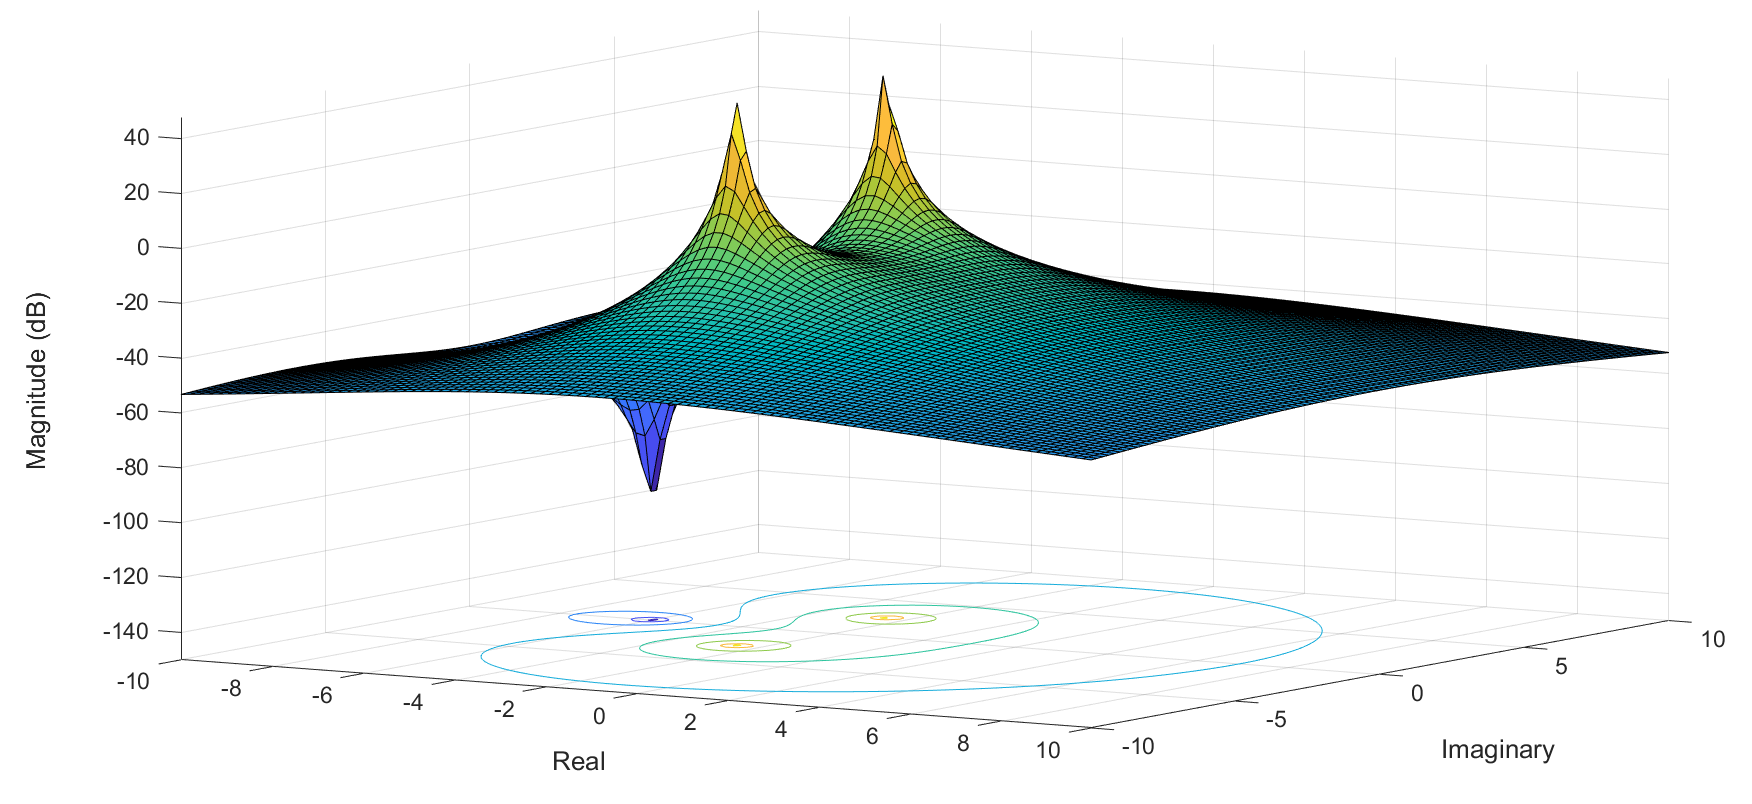
\includegraphics[width=.8\columnwidth]{figures/1_4_magnitude.png}
	\centering
	\caption{Magnitude of the open loop transfer function.}
	\label{fig_3Dmagnitude}
\end{figure}
\begin{figure}[!h]
	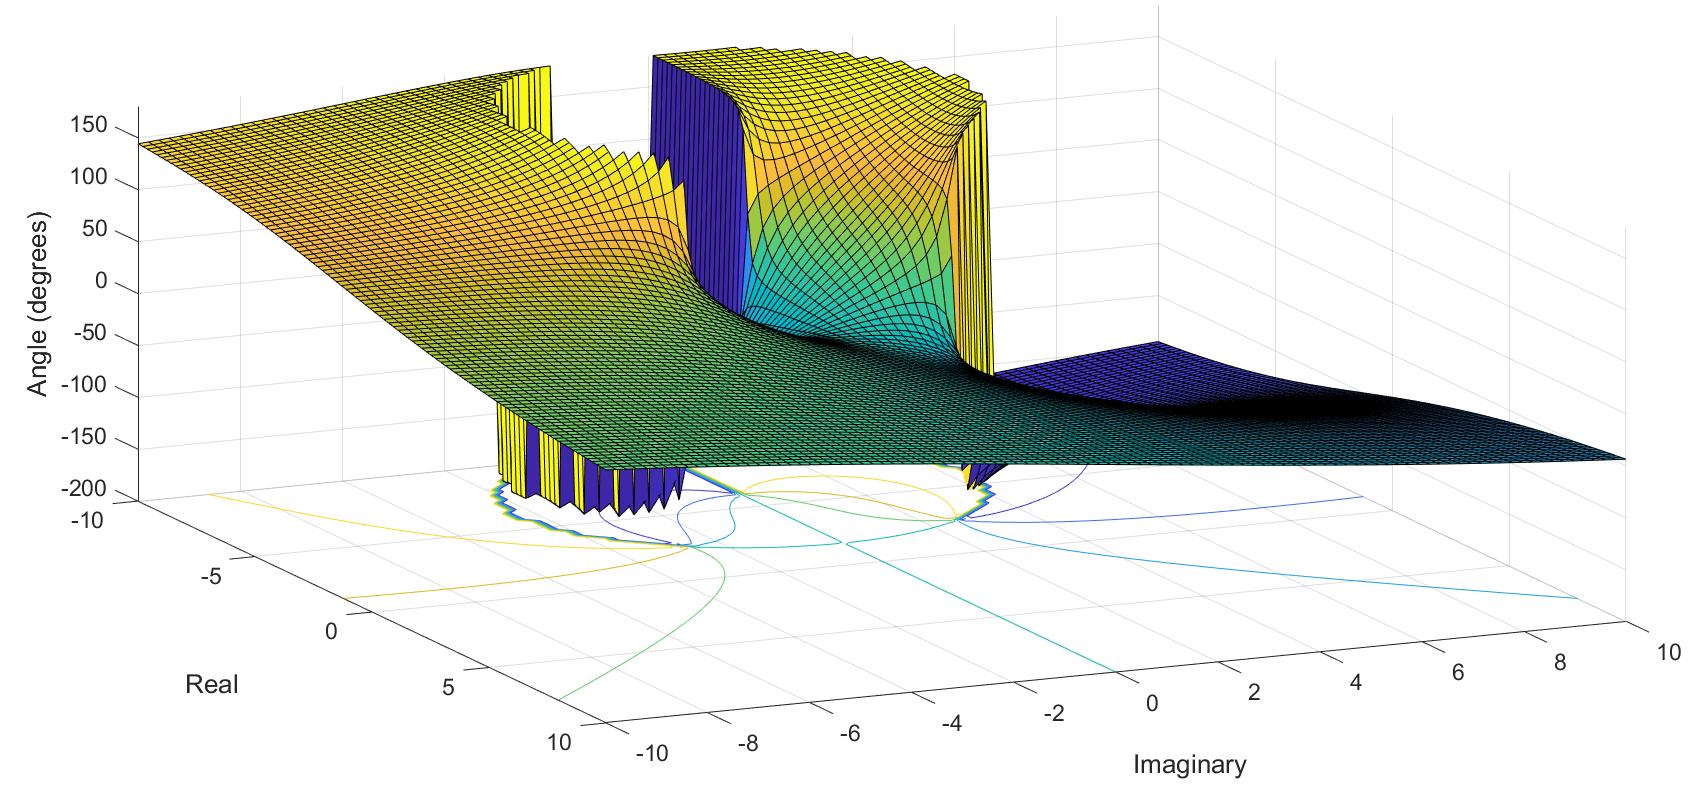
\includegraphics[width=.8\columnwidth]{figures/1_4_phase.png}
	\centering
	\caption{Phase of the open loop transfer function.}
	\label{fig_3Dphase}
\end{figure}
\begin{figure}[!h]
	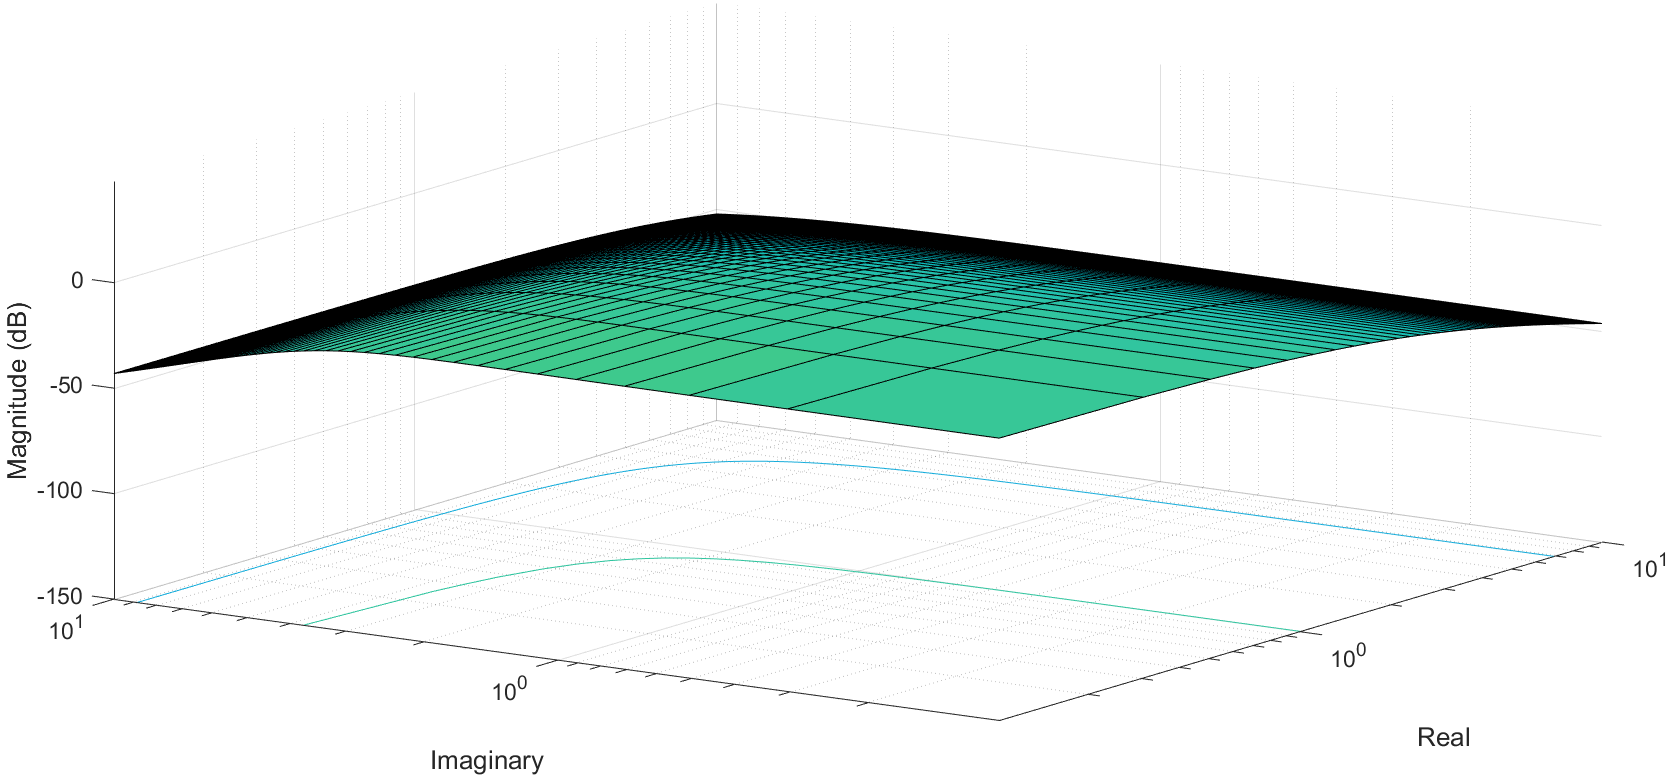
\includegraphics[width=.8\columnwidth]{figures/1_4_magnitudeForBode.png}
	\centering
	\caption{The $3D$ magnitude Bode diagram of the open loop transfer function.}
	\label{fig_magnitudeBode}
\end{figure}
\begin{figure}[!h]
	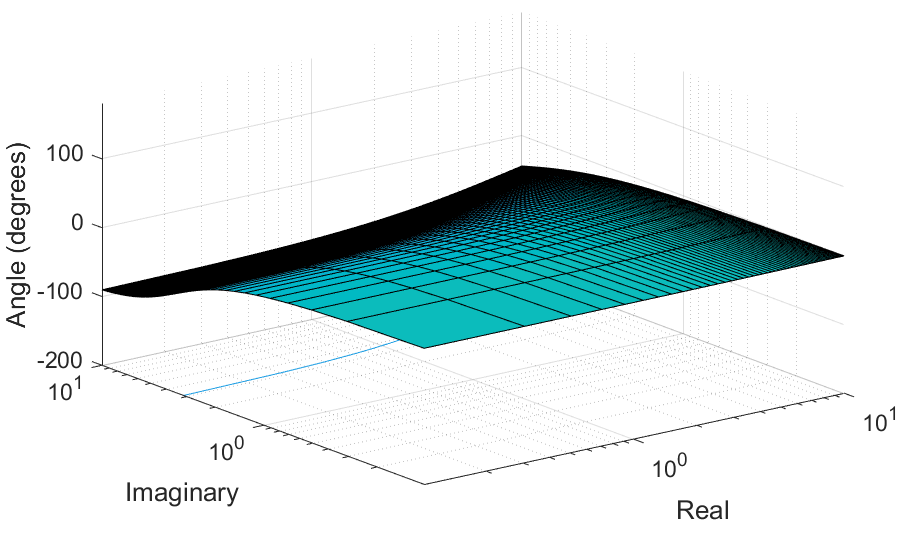
\includegraphics[width=.8\columnwidth]{figures/1_4_phaseForBode.png}
	\centering
	\caption{The $3D$ phase Bode diagram of the open loop transfer function.}
	\label{fig_phaseBode}
\end{figure}
\begin{figure}[!h]
	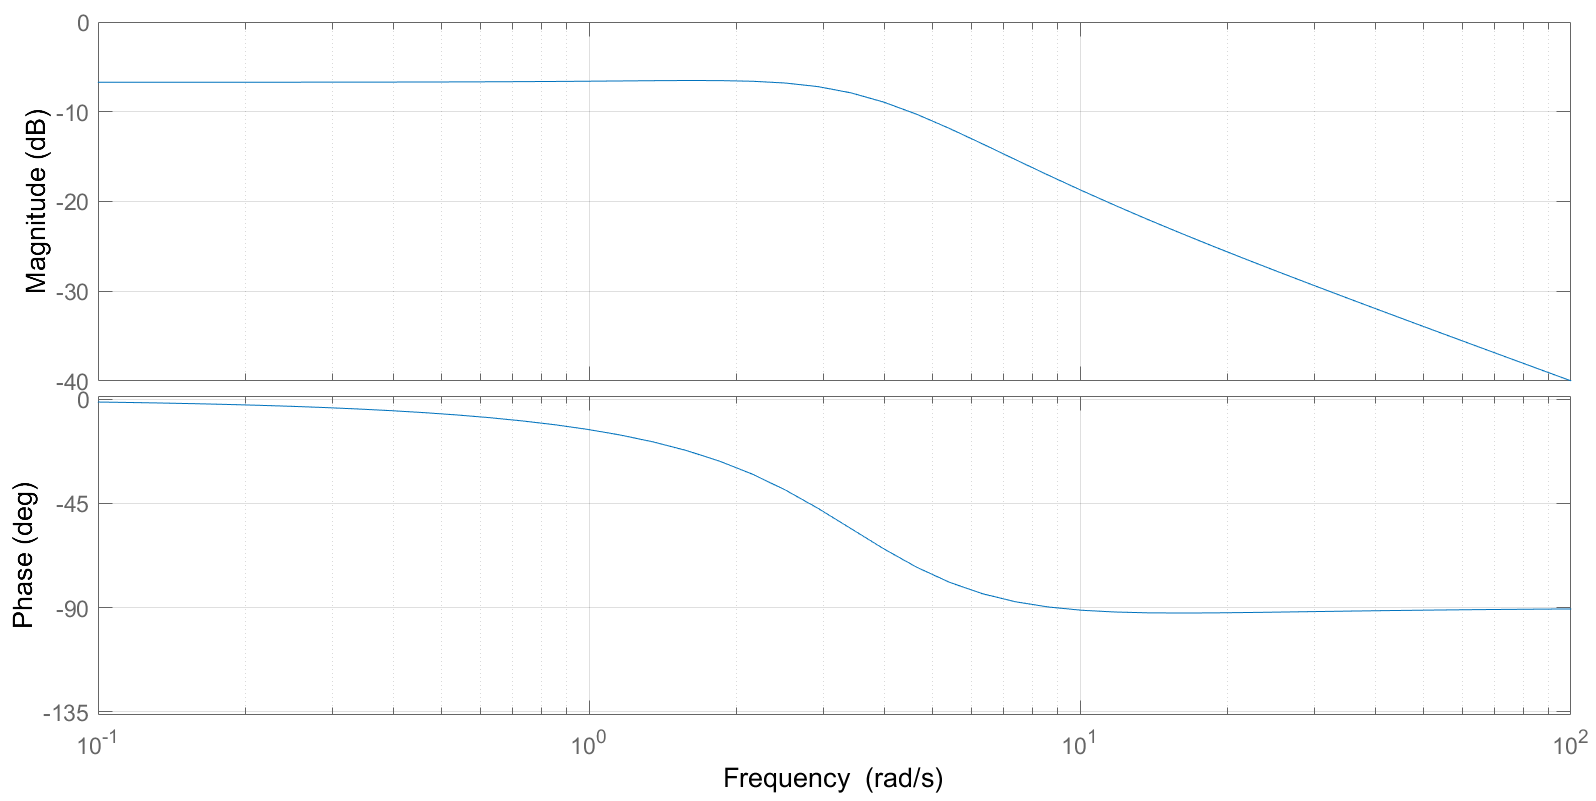
\includegraphics[width=.8\columnwidth]{figures/1_4_bode.png}
	\centering
	\caption{The Bode diagrams of the open loop transfer function.}
	\label{fig_bode}
\end{figure}


\end{solution}

\end{document}


